\chapter{Performance Evaluation}
\label{chap:performance-evaluation}
\vspace{-0.75cm}
\centerline{\rule{149mm}{.02in}}
\vspace{0.75cm}

This section evaluates the performance of the index structures discussed in Chapter \ref{chap:chosen-structures} using their execution times on all the synthetic and real datasets. Execution times are illustrated with plots and bar charts. Tables containing all execution times are available in Appendix \ref{chap:performance-timings}.

Since both point insertion or deletion will have to perform a point query (\texttt{insert} has to check the point is not already stored), point query execution time will not be plotted for some tests. See Appendix \ref{chap:performance-timings} for all point query times.

\begin{figure}
	\makebox[\textwidth][c]{%
		\begin{subfloat}[\texttt{insert}\label{fig:perf-dimensionality-insert}]{%
			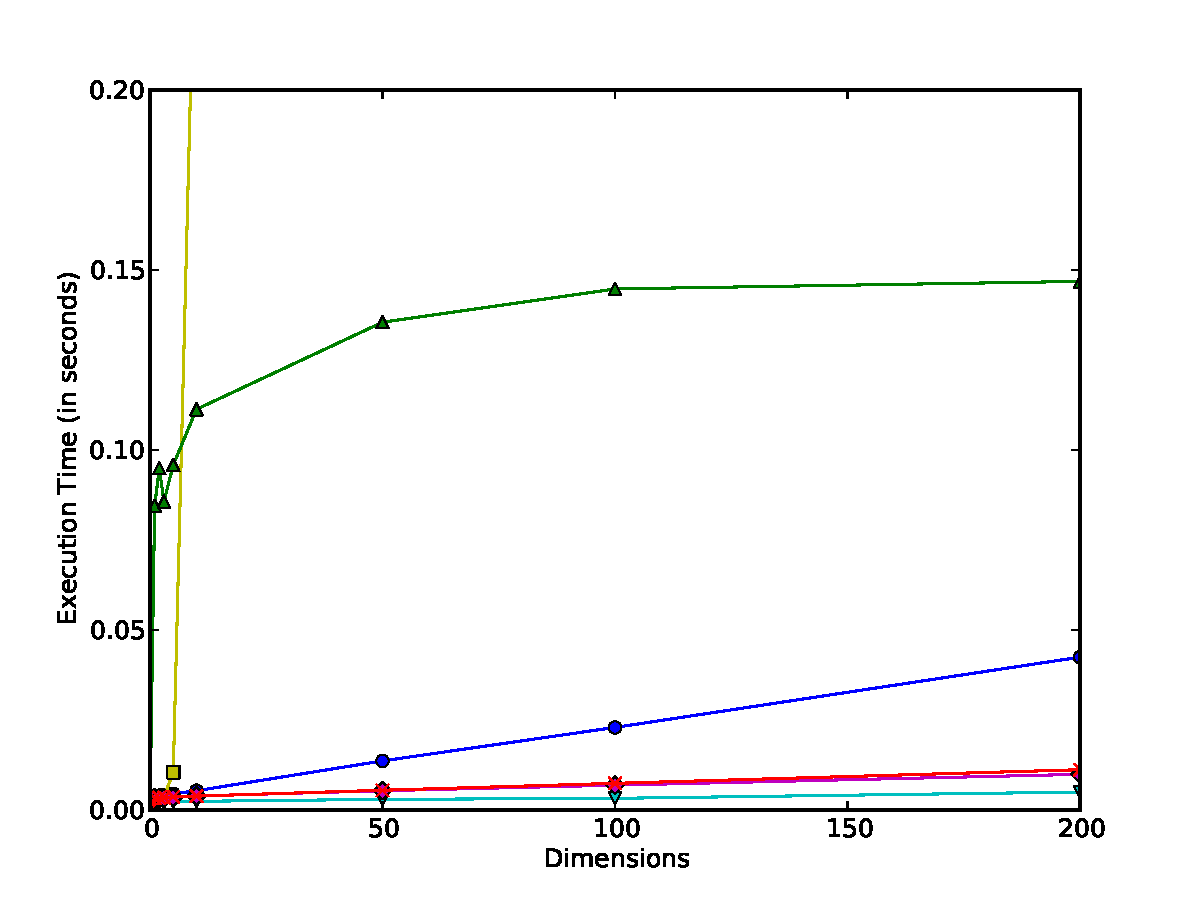
\includegraphics[scale=0.5]{figures/performance_analysis/randuniform_insert_zoomed.pdf}
		}
		\end{subfloat}

		\begin{subfloat}[\texttt{delete}\label{fig:perf-dimensionality-remove}]{%
			\begin{overpic}[scale=0.5]{figures/performance_analysis/randuniform_delete_zoomed.pdf}
				\put(45,33){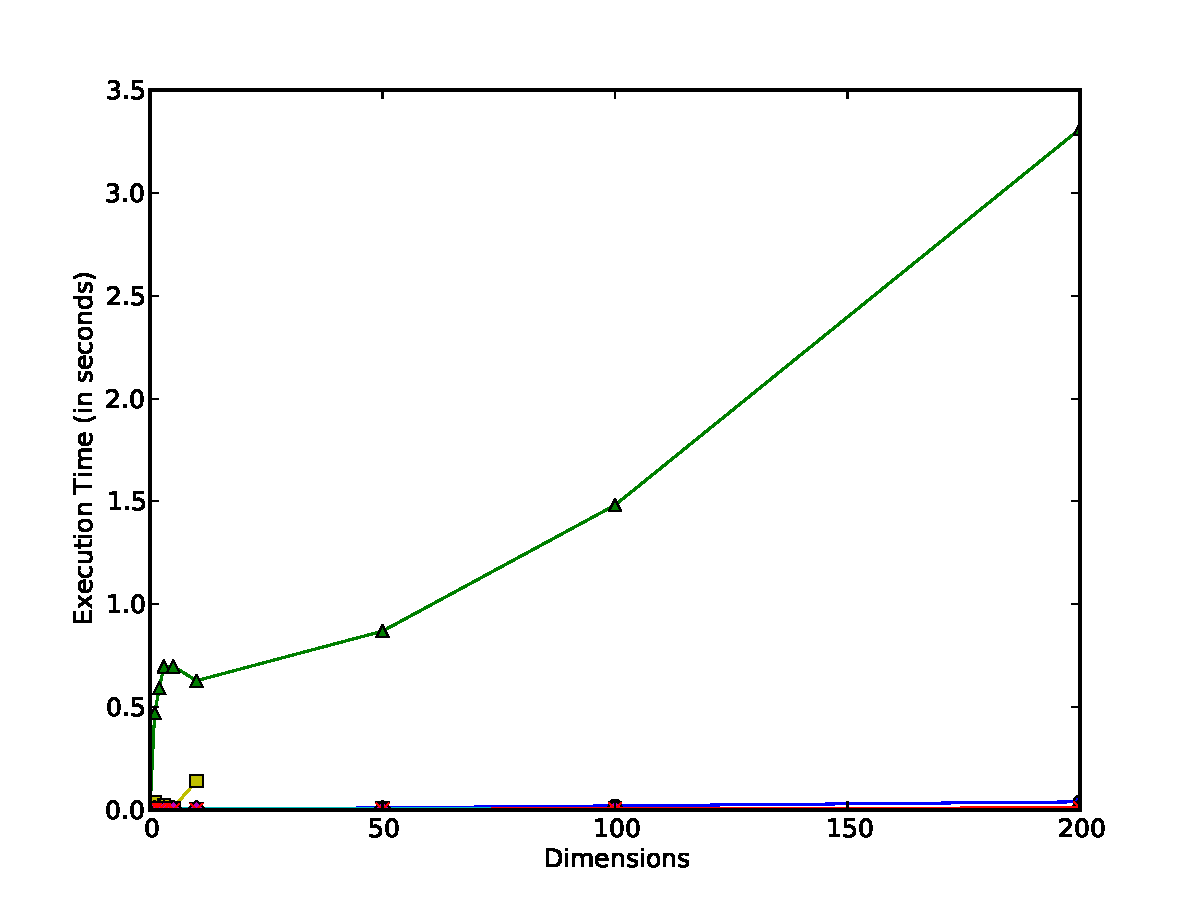
\includegraphics[scale=0.22]{figures/performance_analysis/randuniform_delete.pdf}}
				\put(60,31){\textbf{\sans{Full View}}}
			\end{overpic}
		}
		\end{subfloat}
	}%

	\caption{Structure Performance With Respect To Dimensionality (10,000 Points, Uniform Synthetic Dataset)}
	\label{fig:perf-dimensionality}
\end{figure}

\begin{figure}
	\makebox[\textwidth][c]{%

		\begin{subfloat}[\texttt{insert}\label{fig:perf-size-insert}]{%
			\begin{overpic}[scale=0.5]{figures/performance_analysis/sizevary_insert_zoomed.pdf}
				\put(40,33){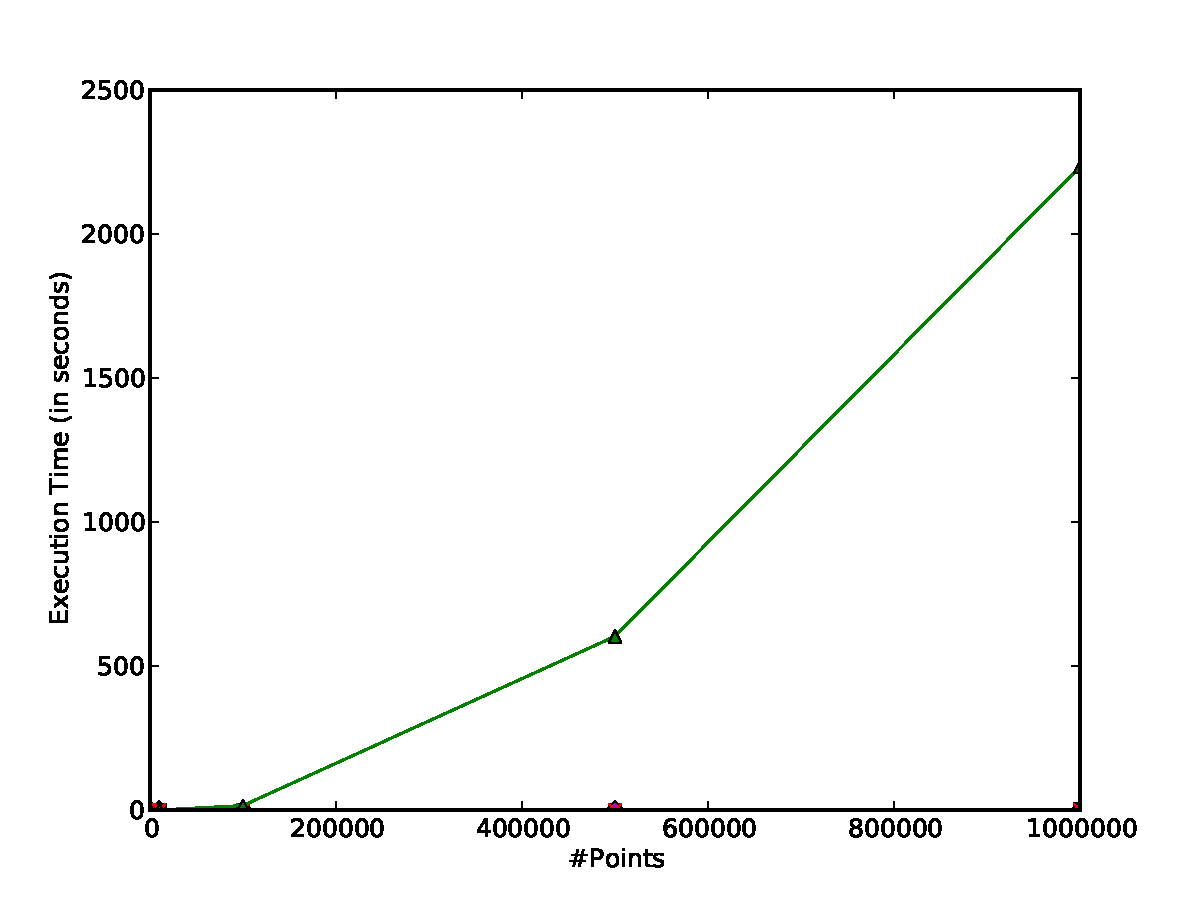
\includegraphics[scale=0.22]{figures/performance_analysis/sizevary_insert.pdf}}
				\put(55,31){\textbf{\sans{Full View}}}
			\end{overpic}
		}
		\end{subfloat}

		\begin{subfloat}[\texttt{delete}\label{fig:perf-size-remove}]{%
			\begin{overpic}[scale=0.5]{figures/performance_analysis/sizevary_delete_zoomed.pdf}
				\put(15,33){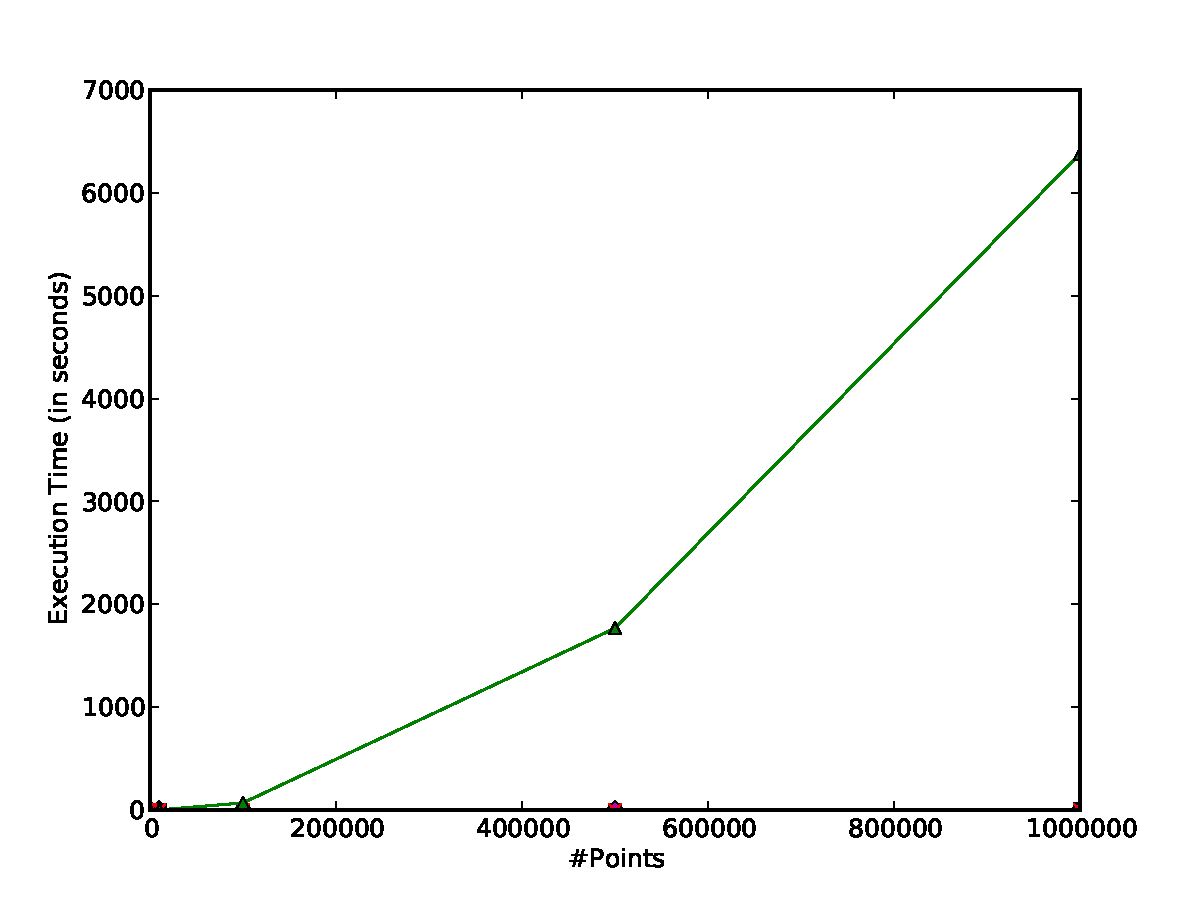
\includegraphics[scale=0.22]{figures/performance_analysis/sizevary_delete.pdf}}
				\put(30,31){\textbf{\sans{Full View}}}
			\end{overpic}
		}
		\end{subfloat}
	}%

	\caption{Structure Performance With Respect To Dataset Size (16D, Uniform Synthetic Dataset)}
	\label{fig:perf-size}
\end{figure}

\begin{figure}
	\begin{picture}(50,50)
		\put(0,-5){\hbox{
			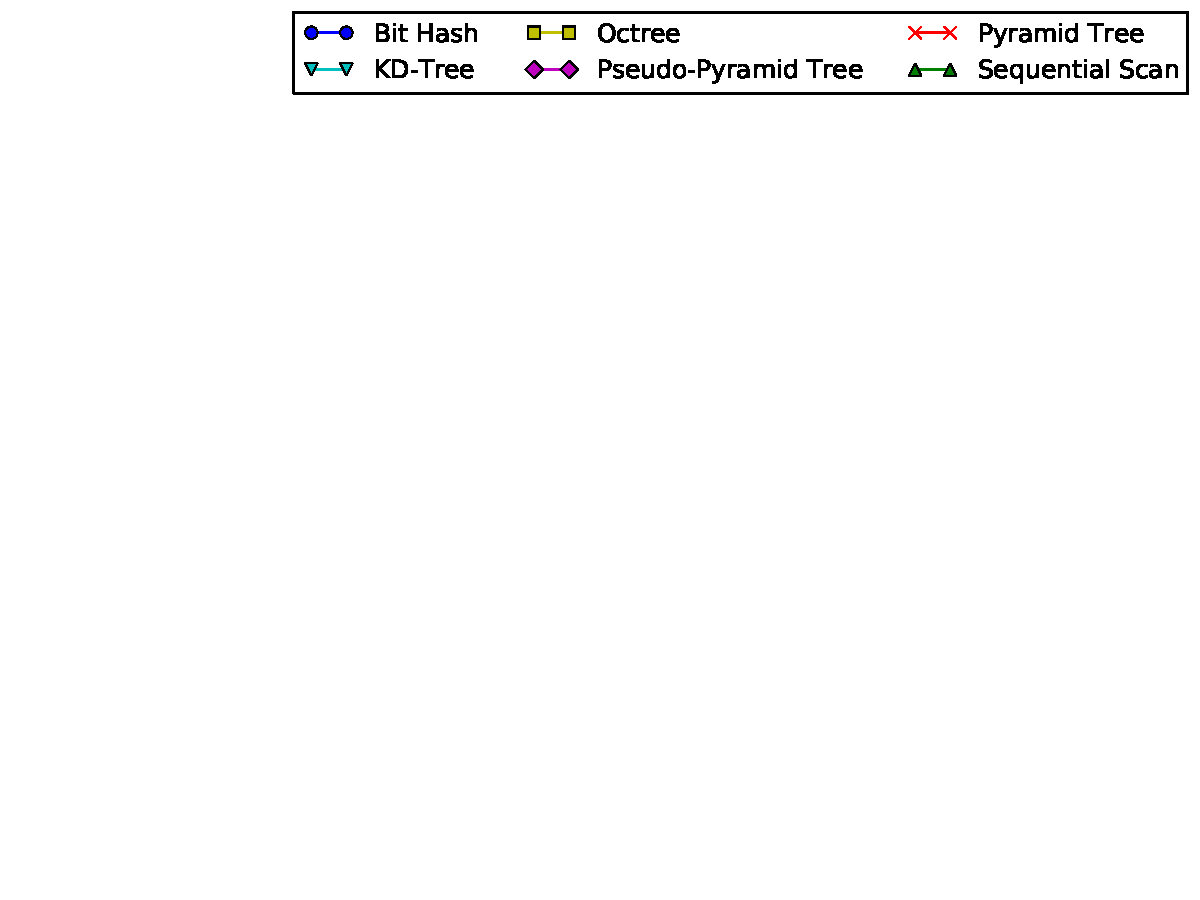
\includegraphics[scale=1.0]{figures/performance_analysis/performance-plots-legend.pdf}
		}}
	\end{picture}
\end{figure}

\section{Dimensionality}

Figure \ref{fig:perf-dimensionality} plots point \textit{dimensionality} against execution time of \texttt{insert} and \texttt{delete} operations for each structure. It shows that the performance of all structures gets worse as $d$ increases, but the rate performance decreases varies. For insertions, sequential scan quickly becomes slower as $d$ decreases, but the decrease starts to tail off as $d$ gets higher. For example, there is little different between \texttt{insert} execution time when the dimensions increase from 100 to 200. \texttt{delete} is sensitive to $d$, with its execution time increasing much faster as $d$ increases. This is because more data must be moved and de-allocated when performing array deletion, because there is more data per point. \texttt{insert} pre-allocates memory up-front, so having more data per point has less of an impact on performance.

Octree execution time exponentially increases with $d$, as shown by the plots. When $d > 10$, the sheer amount of nodes needed when sub-dividing space causes the structure to run out of memory. From this we can conclude that this structure is not suitable for high-dimensional data.

All three hash-based structures use an $O(d)$ hashing function, but the constant factors in each are different. Execution times of Bit Hash, Pseudo-Pyramid Tree and Pyramid Tree all increase linearly with $d$, but Bit Hash has a greater slope. Pseudo-Pyramid Tree has the cheapest hash function and as such, is the fastest of the three structures as $d$ increases.

There have been discussions regarding the $kd$-tree's unsuitability for high-dimensional data in the literature \cite{highd-nn, search-highd-analysis}. However, the $kd$-tree is affected the least by dimensionality in these tests, which was initially surprising. However, the structure does not have an explicit $O(d)$ computation; its best and worst running times are $O(\log_2 n$) and $O(n)$ respectively. Therefore, as long as the tree remains balanced, dimensionality will have little impact on the $kd$-tree's performance.

\section{Dataset Size}

Figure \ref{fig:perf-size} plots dataset \textit{size} against execution time of \texttt{insert} and \texttt{delete} operations for each structure. Sequential scan is clearly not scalable to large dynamic datasets, taking over 2000 seconds to incrementally construct a structure to store 1,000,000 unique points and over 6000 seconds to incrementally delete the points. The octree ran out of memory quickly, since 16-dimensional points are used. Again, this shows the octree is unsuitable for high-dimensional data.

Figure \ref{fig:perf-dimensionality} shows the $kd$-tree is the fastest with 10,000 points, but it becomes the slowest (barring sequential scan) as dataset size increases. \texttt{delete} becomes even slower than \texttt{insert} does as $n$ increases, with deletions being two times slower than insertions with 1,000,000 points. This is a problem if an application removes individual points from the structure frequently.

The Pseudo-Pyramid Tree and Bit Hash have the fastest and slowest hashing functions respectively. This again affects the performance of the structures, with the Pseudo-Pyramid Tree being the fastest for both operations and Bit Hash being the slowest. These tests show that three hash-based structures are the most scalable structures out of the implemented in this project. As more synthetic data is given to the structures, execution time of the hash-based structures increases much slower than the point $kd$-tree or sequential scan.

\section{Real Data}
\label{sec:real-dataset-times}

\begin{figure}
	\makebox[\textwidth][c]{%
		\begin{subfloat}[\label{fig:perf-real-astrophyiscs}]{%
			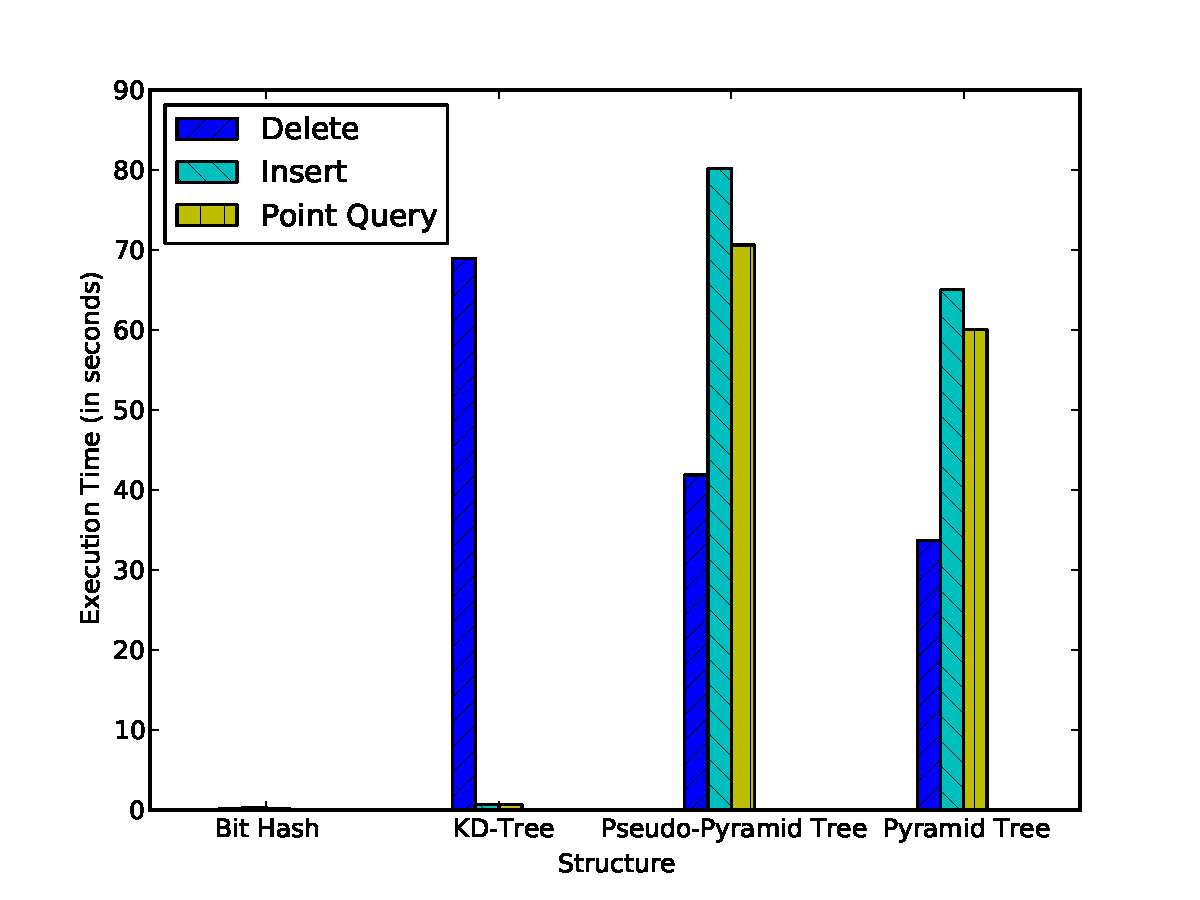
\includegraphics[scale=0.5]{figures/performance_analysis/astrophysics_times.pdf}
		}
		\end{subfloat}
		\begin{subfloat}[Sampled Hurricane Isabel (500,000 Points)\label{fig:perf-real-hurricane}]{%
			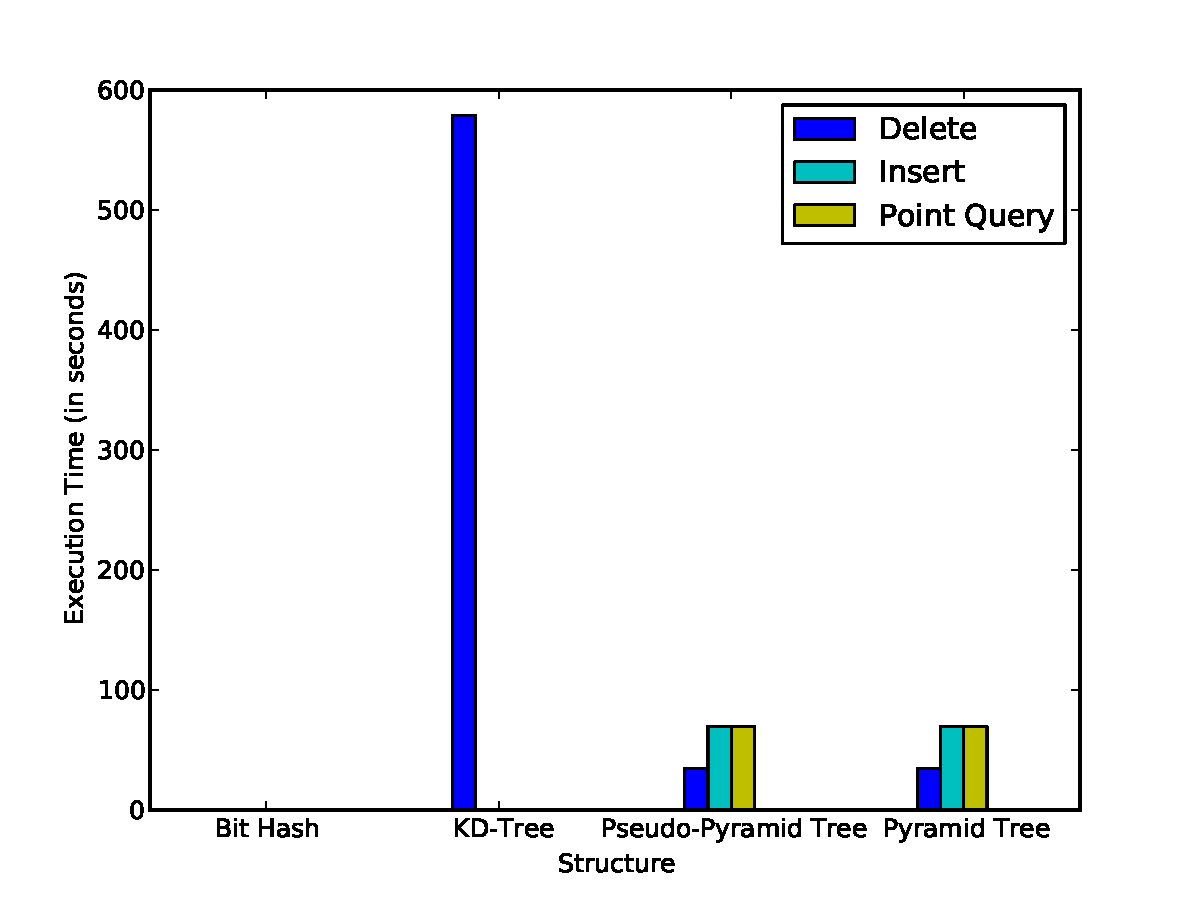
\includegraphics[scale=0.5]{figures/performance_analysis/hurricane_times.pdf}
		}
		\end{subfloat}
	}%

	\makebox[\textwidth][c]{%
		\begin{subfloat}[Zoomed Sampled Astrophysics\label{fig:perf-real-astrophysics-zoomed}]{%
			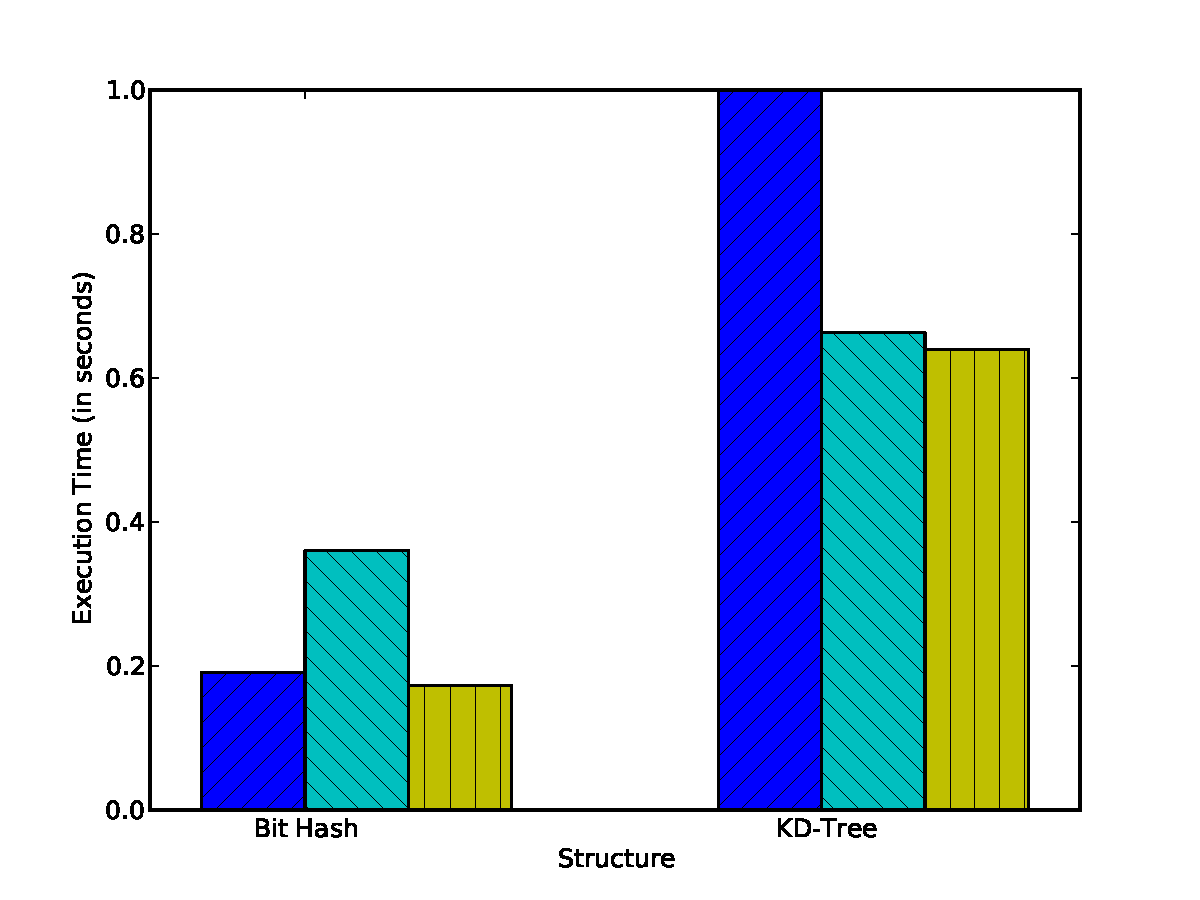
\includegraphics[scale=0.275]{figures/performance_analysis/astrophysics_times_zoomed.pdf}
		}
		\end{subfloat}
		\begin{subfloat}[Zoomed Sampled Hurricane Isabel\label{fig:perf-real-hurricane-zoomed}]{%
			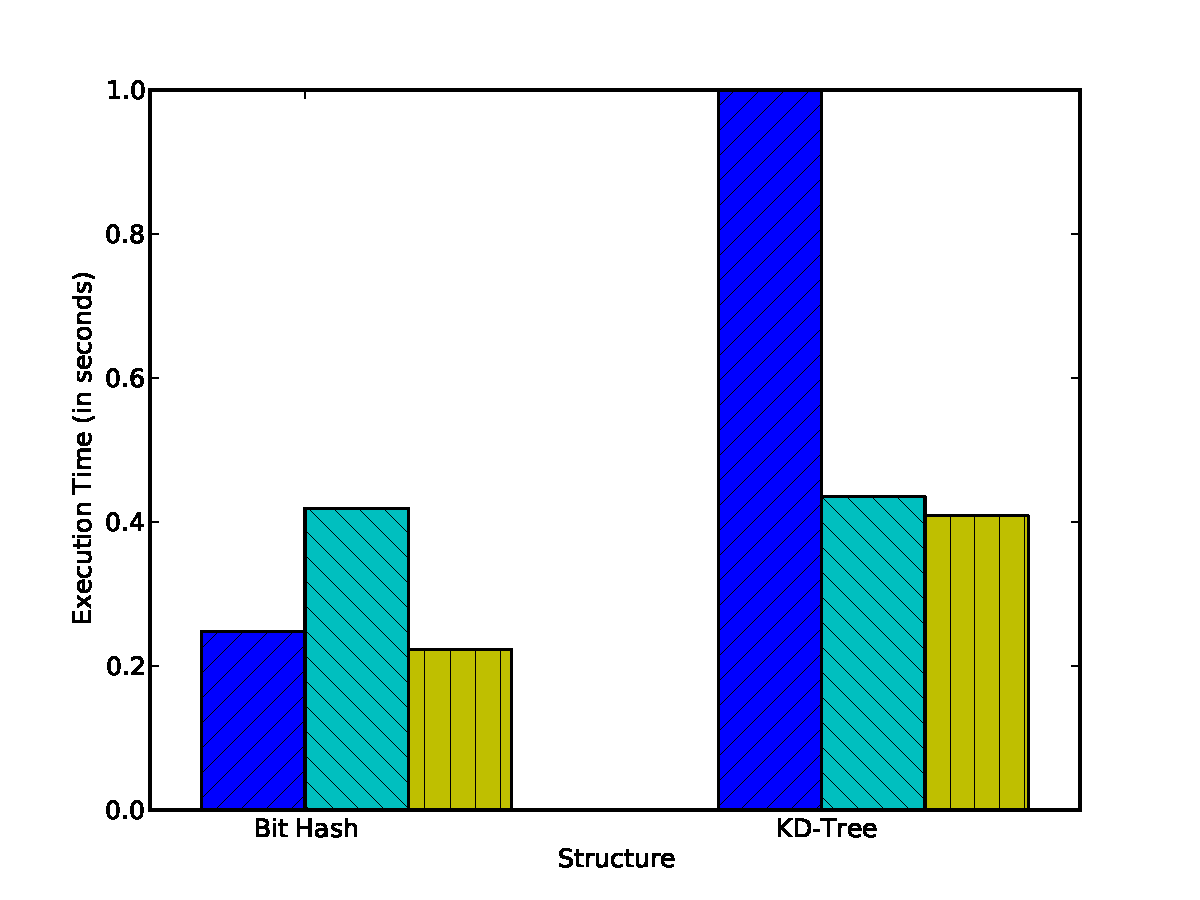
\includegraphics[scale=0.275]{figures/performance_analysis/hurricane_times_zoomed.pdf}
		}
		\end{subfloat}
	}%

	\makebox[\textwidth][c]{%
		\begin{subfloat}[Armadillo Mesh (435,544 Points)\label{fig:perf-real-armadillo}]{%
			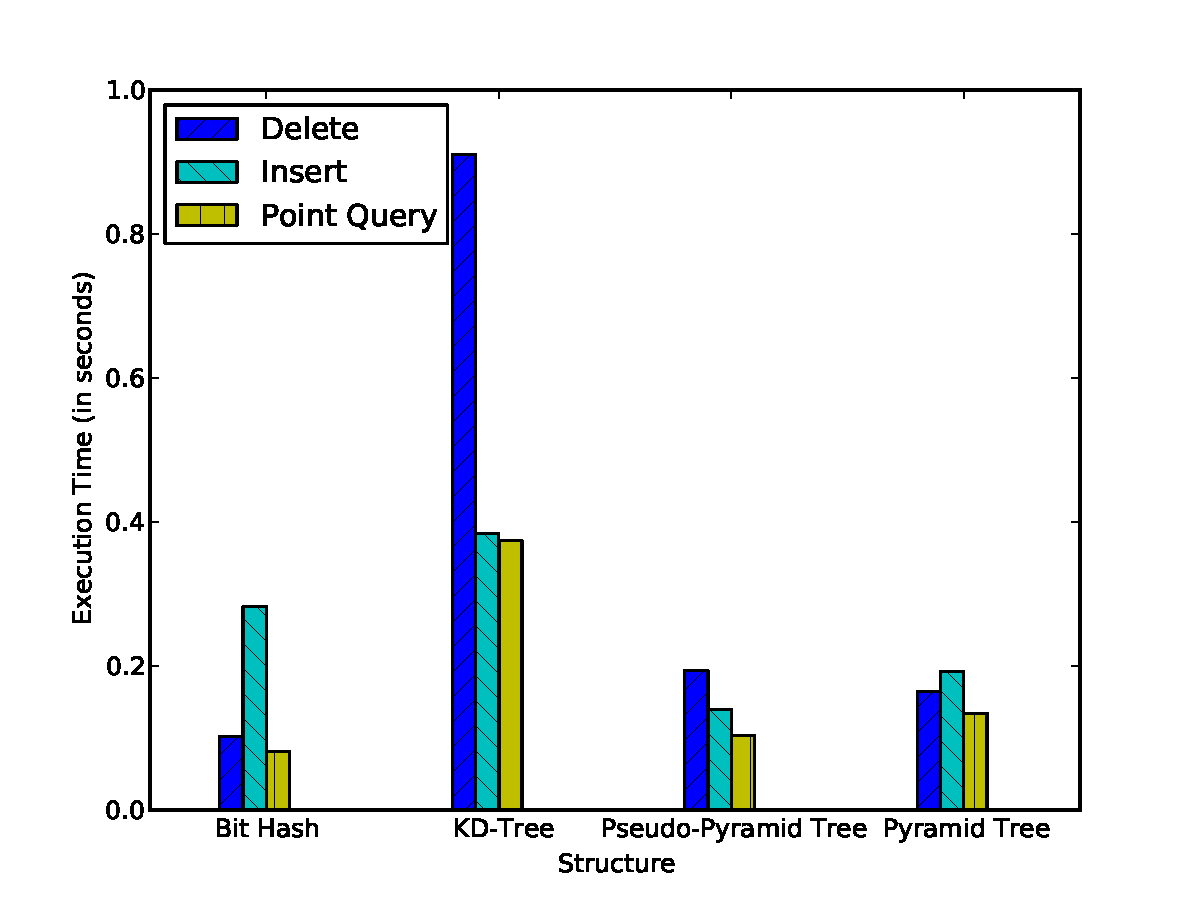
\includegraphics[scale=0.5]{figures/performance_analysis/armadillo_times.pdf}
		}
		\end{subfloat}
	}%
	\caption{Structure Performance on Real Datasets}
	\label{fig:perf-real}
\end{figure}

Figure \ref{fig:perf-real} illustrates index structure performance of each operation on the three real datasets. Sequential scan is not shown because performance is similar to that shown in the dataset size plots in Figure \ref{fig:perf-size}. See Table \ref{tab:perf-real} in Appendix \ref{chap:performance-timings} for all execution times on the real datasets.

Bit Hash outperforms all structures for point queries and deletion on all three datasets. It has the fastest insertion time as well, except for the armadillo mesh where the Pseudo-Pyramid Tree and Pyramid Tree beats it. Profiling revealed that Bit Hash performs more memory allocations for insertions, which is the reason it is slower than point deletions or queries. Bit Hash is significantly faster than the other hash-based approaches on the astrophysics and hurricane Isabel dataset, with queries being over 400 and 198 times faster than the Pyramid Tree respectively.

$kd$-trees vastly outperform Pseudo-Pyramid Tree and Pyramid Tree and almost match Bit Hash's speed. However, individual point deletion is slow. It took almost 580 seconds to delete each point from the hurricane dataset. It is interesting see that the Pyramid Tree was faster than Pseudo-Pyramid Tree for the astrophysics dataset, but over two times slower with the hurricane dataset. The hashing functions appear to be highly sensitive to data distribution. This will be explored in the next section.

\section{Impact of Bucket Size}

Pyramid Tree point queries are approximately 7.26 times faster than sequential scan with the astrophysics dataset and 14.76 times faster with hurricane Isabel. With the armadillo mesh, Pyramid Tree queries are \textit{1580} times faster. The speedup varies massively between datasets. Considering algorithms which perform queries in $O(\log n)$ time exist, this raises an important question: why is the Pyramid Tree so slow with some datasets?

Bit Hash is the fastest structure, but the Pyramid Tree is the slowest. Both structures user the same underlying hash table implementation. Therefore, the performance differences must be caused by how the structures reduce points to a one-dimensional value. 

Despite hashing a point taking $O(d)$ time, point queries will take much longer if buckets contain many points. If each bucket contains exactly one point, then operation execution time approaches $O(d)$. On the other extreme, where a single bucket contains all points, the complexity becomes $O(n)$. The number of points in a bucket, or \textit{bucket size}, is one of the most important factors to consider when analysing the performance of hash-based index structures. A ``good" hashing function tries to achieve an amortised running time of $O(d)$ by ensuring very few points are mapped to the same bucket.

\begin{table}
	\centering
	\makebox[\textwidth][c]{%
		\begin{tabular}{|l|l|l|l|l|}
			\hline
			& & \multicolumn{3}{c|}{\textbf{Bucket Statistics}} \\
			\hline
			\textbf{Dataset} & \textbf{Time to Query (sec)} & \textbf{Average} & \textbf{Max} & \textbf{\#Buckets} \\
			\hline
			\textbf{Pseudo-Pyramid Tree} & & & & \\
			500,000 16D Random Points & 0.105091 & 1.02395 & 4 & 488304 \\
			500,000 Astrophysics Points & 70.4391 & 62500 & 153471 & 8 \\
			500,000 Hurricane Isabel Points & 14.3358 & 1262.63 & 154979 & 396 \\
			435,544 3D Armadillo Mesh Points & 0.141219 & 19.1465 & 187 & 22748 \\
			\hline
			\textbf{Pyramid Tree} & & & & \\
			500,000 16D Random Points & 0.177153 & 1.16286 & 7 & 429974 \\
			500,000 Astrophysics Points & 60.0216 & 3521.13 & 235260 & 142 \\
			500,000 Hurricane Isabel Points & 44.1224 & 4065.04 & 354965 & 123 \\
			435,544 3D Armadillo Mesh Points & 0.13448 & 2.45938 & 1173 & 177095 \\
			\hline
			\textbf{Bit Hash} & & & & \\
			500,000 16D Random Points & 0.249102 & 1.00975 & 3 & 495172 \\
			500,000 Astrophysics Points & 0.172516 & 1.01051 & 5 & 494800 \\
			500,000 Hurricane Isabel Points & 0.222288 & 1.00861 & 3 & 495733 \\
			435,544 3D Armadillo Mesh Points & 0.0811833 & 1.00891 & 3 & 431696 \\
			\hline
		\end{tabular}
	}%
	\caption{Statistics on Bucket Size, Based on Dataset, of All Hash-Based Structures}
	\label{tab:perf-bucket-stats}
\end{table}

Table \ref{tab:perf-bucket-stats} shows the average and maximum bucket size, as well as how many buckets there are, for the real datasets and a uniformly distributed synthetic dataset. The table shows there is a relationship between bucket size and speed -- higher average bucket sizes are paired with longer execution times. 

The Pyramid Tree stores 235,260 points from the astrophysics dataset in a \textit{single} bucket, meaning up to 235,260 points will be scanned when performing a query. Both the Pyramid and Pseudo-Pyramid Tree essentially degenerate to a \textit{semi-sequential scan} with the scientific datasets. Bit Hash's average bucket size is very close to 1, meaning only one point must be scanned for most operations. Larger average bucket size means queries require more computation on average. The Pyramid Tree and Pseudo-Pyramid Tree are much faster on the synthetic dataset and the armadillo mesh than the two scientific datasets. Table \ref{tab:perf-bucket-stats} shows how average bucket size is much lower for these datasets when compared to the two scientific datasets. This shows that, given certain point distributions, these structures can be fast.

Ideally, the number of buckets is equal to the number of points, meaning average bucket size is 1. This is known as \textit{perfect hashing}. Bit Hash shows that consistently good performance can be achieved when the average bucket size tends to one. Unfortunately, Bit Hash is unreliable because it is highly susceptible floating-point errors. If a more reliable hashing function that achieves close to 1 average bucket size, then significant increases in point query performance can be achieved.

\section{Impact of Tree Balance}

While the difference in performance is less drastic than the hash-based structures, the point $kd$-tree's performance still varies between datasets. $kd$-tree point queries for 500,000 points sampled from astrophysics dataset took 0.639265 seconds, but only 0.374425 on the armadillo mesh. The cause of this is most likely the \textit{balance} of the tree. Skewed datasets are known to affect the balance of spatial decomposition trees, resulting in longer paths from the root node to the leaves.

To investigate this further, the \textit{balance factor} of the point $kd$-tree has been measured. The balance factor is defined as the \textit{average} length of a path from the root to a leaf \cite{kdtree-v-bdtree}. A lower balance factor means the $kd$-tree has to visit less nodes on average when performing a point query, so queries will be faster. A $kd$-tree is balanced when its balance factor is $\log_2 n$. When $n = 500,000$, the best possible balance factor is $\log_2 (500,000) \approx 19$.

The \textit{exact match query cost}, used to evaluate $kd$-tree variations by Dandamudi and Sorenson \cite{kdtree-v-bdtree}, represents the average number of points visited in the tree for a point query. Higher exact match query cost means the tree has to do more work on average to find a point, making the structure slower. This will be measured alongside balance factor to determine the average work required per operation.

Table \ref{tab:kdtree-balance-factor} contains the balance factor, exact match query cost and maximum path length from the root to a leaf when different point distributions are stored in the tree. It shows exact match query cost increases with the balance factor. Therefore, as the balance factor increases, performance decreases.

\begin{table}
	\centering
	\makebox[\textwidth][c]{%
		\begin{tabular}{|l|l|l|l|}
			\hline
			\multicolumn{1}{|c|}{\textbf{Dataset}} & \centrespecialcell{\textbf{Balance} \\ \textbf{Factor}} & \centrespecialcell{\textbf{Max Path} \\ \textbf{Length}} & \centrespecialcell{\textbf{Exact Match} \\ \textbf{Query Cost}} \\
			\hline
			\leftspecialcell{Random 10D Points \\ (Uniform Distribution)} & 24.8285 & 47 & 24.4968 \\
			\leftspecialcell{Random 10D Points \\ (Skewed Distribution)} & 24.9092 & 44 & 24.5714 \\
			\leftspecialcell{Random 10D Points \\ (Clustered Distribution)} & 30.3362 & 57 & 29.9911 \\
			Astrophysics & 32.405 & 120 & 29.7373 \\
			Hurricane Isabel & 47.7236 & 123 & 40.5602 \\
			\hline
		\end{tabular}
	}%
	\caption{Point $kd$-tree Balance Factor and Exact Match Query Cost with 500,000 Points from Various Datasets}
	\label{tab:kdtree-balance-factor}
\end{table}

While the $kd$-tree does not degenerate to semi-sequential scan when processing datasets with skew, like the Pyramid Tree, these results show that these datasets do affect the structure's overall performance. For this reason, many variants of the $kd$-tree have been developed in an attempt to reduce the balance factor with skewed datasets. Examples of such variants include the BD-Tree \cite{kdtree-v-bdtree} and fair split tree\cite{fair-split-tree}. Appendix \ref{chap:additional-structures} discusses initial performance results of a $kd$-tree variant implemented in this project. This variant was not explored in more detail due to project time constraints.

\section{Memory Overhead}

The memory consumption of each structure has been recorded alongside execution time. If a structure's memory footprint is large, it may not scalable to large datasets. 32-bit floating point numbers are used in this project, so the minimum amount of memory required to store 500,000 points from the 16D synthetic dataset and the 10D astrophysics dataset is 30.52MB and 19.07MB respectively.

Table \ref{tab:memory-overhead} shows the memory used by each structure. The \textit{overhead factor} is also provided, which measures how much additional memory is needed to store the points. For example, an overhead factor of 1 would mean there is no overhead. A factor of 2 would mean \textit{twice} the minimum amount of memory is used. The memory overhead of the structures with a synthetic and real dataset are shown. Similar results were found with the other test datasets, so for brevity they are not shown. Octree runs of memory, so no measurements are provided for it.

\begin{table}
	\centering
	\begin{tabular}{|r|l|l|l|l|}
		\hline
		& \multicolumn{2}{|c|}{\textbf{16D Synthetic Data (Uniform)}} & \multicolumn{2}{|c|}{\textbf{10D Astrophysics}} \\ 
		\hline
		\textbf{Structure} & \multicolumn{1}{|c|}{\textbf{Memory Usage}} & \multicolumn{1}{|c|}{\textbf{Overhead}} & \multicolumn{1}{|c|}{\textbf{Memory Usage}} & \multicolumn{1}{|c|}{\textbf{Overhead}} \\
		\hline
		Sequential Scan & 30.53MB & 1.000327 & 19.074MB & 1.000327 \\
		Pseudo-Pyramid Tree & 51.53MB & 1.688401 & 20.98MB & 1.099984 \\
		Pyramid Tree & 42.493MB & 1.392300 & 20.99MB & 1.100508 \\
		Bit Hash & 54.86MB & 1.797509 & 43.42MB & 2.276516 \\
		$kd$-tree & 38.15MB & 1.25 & 26.7MB & 1.399884 \\
		\hline
	\end{tabular}
	\caption{Memory Overhead of Structures When Storing 500,000 Points from Different Datasets}
	\label{tab:memory-overhead}
\end{table}

Sequential scan incurs almost no overhead since only three extra pointers are used by the underlying resizeable array. The point $kd$-tree produces the next lowest overhead. Each point in the tree incurs 8/16 bytes of overhead, since they are stored in a node that contains pointers to its two children. 

The overhead incurred by the hash-based structures depends on the dataset. Each bucket adds overhead, so memory overhead is larger if there are many buckets. For execution speed, it is ideal to have one bucket for each point, but this consumes more memory. The Pseudo-Pyramid Tree maps all points in the astrophysics dataset to only 8 buckets and the structure's overhead factor is 1.099984. The structure uses 493,488 buckets for the synthetic data and has an overhead factor of 1.688401. Notice how the overhead factor is much higher. Bit Hash tends to use one bucket for each point, so it consumes the most memory out of all the structures. While perfect hashing is desirable for speed, it can cause problems if large datasets must be processed on memory constrained systems. If memory is a limited resource, then the point $kd$-tree may be a more suitable structure because it has comparatively low overhead that is not dependent on point distribution.

\section{Conclusion}

The performance evaluation performed in this chapter has revealed the following:
\begin{itemize}
	\item Sequential Scan is not scalable to large datasets
	\item the standard octree is not usable for high-dimensional data
	\item Pseudo-Pyramid Tree and Pyramid Tree degenerate to semi-sequential scan with the two scientific datasets, but perform well with the armadillo mesh and synthetic datasets
	\item point $kd$-tree speed is affected by point distribution, but not as much as hash-based structures
	\item the point $kd$-tree outperforms the Pseudo-Pyramid Tree and Pyramid Tree on real scientific datasets
	\item individual point deletion with the point $kd$-tree is highly inefficient
	\item if near perfect hashing is achieved, then a structure faster than the point $kd$-tree has been found
	\item hash-based structures use more memory than point $kd$-trees, with overhead increasing as they get closer to perfect hashing
	\item hash-based structures with near perfect hashing might not be suitable for large datasets if low memory consumption is a priority
\end{itemize}

The point $kd$-tree is consistently slower than Bit Hash with the real datasets. However, the $kd$-tree is more reliable because it does not use a hashing function that is highly susceptible to floating point error. Bit Hash shows perfect hashing is a desirable property, but it will not be discussed further in the project because of its unreliability.